\documentclass[12pt,a4paper]{article}

\usepackage[utf8]{inputenc}
\usepackage[T1]{fontenc}
\usepackage{lmodern}

\usepackage{graphicx}
\usepackage{microtype}
\usepackage{hyperref} 
\usepackage[frenchb]{babel}

\usepackage{listings}	   
\lstdefinestyle{customstyle}{
    basicstyle=\footnotesize,
    breakatwhitespace=false,         
    breaklines=true,                 
    captionpos=b,                    
    keepspaces=true,                                                                                       
    tabsize=4,
    frame=single,
    moredelim=[is][\underbar]{_}{_}
}
\lstset{style=customstyle}

\title{MGS plugin framework manual}
\author{Antoine Forgerou \and Jérémy Bardon}
\date{}
	
\begin{document}
	\renewcommand{\contentsname}{Sommaire}
	\renewcommand{\arraystretch}{1.8}
	\maketitle	
	
	\vspace{0.80cm}
	\tableofcontents	

	\thispagestyle{empty}	
	\setcounter{page}{0}
	\newpage
	
\begin{abstract}
Le framework MGS permet de gérer de manière transparente la modularité des 
applications basées sur l'utilisation de plugins. 
\\\\
Plutôt que d'obliger les utilisateurs à remplir de long fichiers de configurations, 
nous avons choisi le plus possible de nous concentrer sur une architecture de 
fichier la moins contraignante possible.
\end{abstract}

\section{Recommandations et pré-requis}
L'ensemble du framework et des plugins sont tous gérés sous la forme de projets 
\emph{maven}. Il est donc nécessaire d'avoir cet outil installé pour développer 
la plateforme.
\\\\
Notez qu'il est tout à fait possible d'utiliser le framework sous forme de d'archive 
\emph{jar} pour l'inclure dans un projet n'utilisant pas \emph{maven}. Le choix de 
maven permet de faciliter l'intégration des dépendances entre la plateforme, les 
plugins principaux et les plugins secondaires.
\\\\
Pour des raisons de clarté, tout les chemins indiqués dans ce manuel ont pour racine 
le dossier du projet \emph{snake} cloné depuis GitHub.

\section{Installation}
Cette section explique comment installer la plateforme localement et y ajouter 
les plugins développés par l'équipe pour l'exemple du snake. La plupart des commandes 
ne seront pas expliquées ici mais l'installation des plugins est détaillée dans la 
section suivante.

\subsection{Récupérer le projet et installer la plateforme}
Le projet est hébergé sur GitHub, pour le récupérer il suffit de le cloner avec
la commande suivante :

\begin{lstlisting}[language=bash,caption=Télécharger le projet]
$ git clone https://github.com/masters-info-nantes/snake.git
\end{lstlisting}

Pour installer la plateforme localement, il faut utiliser la commande 
\og{}\emph{mvn install}\fg{} dans la répertoire de la plateforme à savoir 
\emph{/platform}.

Ceci va avoir pour effet de rendre disponible la plateforme pour les plugins 
que nous allons compiler dans l'étape suivante.

\subsection{Configuration de la plateforme}
Il existe un seul fichier de configuration qui permet d'ajuster le fonctionnement 
du framework. Ce fichier se nomme \emph{settings.txt} et se trouve dans le 
répertoire \emph{/platform/resources}.

\begin{table}[h]
\centering
	\begin{tabular}{lp{9cm}}
		pluginspath & Chemin absolu ou relatif vers le dossier qui contient tout les plugins.\\
					 
		startplugin & Nom du plugin\footnote{Il s'agit du nom du dossier du 
		plugin} à charger au démarrage. Obligatoirement runnable.\\	
		
		debug & Lance l'inspecteur de la plateforme qui liste les plugins si la valeur 
		est égale à \emph{true}				 
	\end{tabular}	
\caption{Paramètres du fichier settings.txt}
\end{table}
	
Ce répertoire contient également un dossier \emph{plugins} qui rassemble les fichiers 
\emph{jar} des plugins développés par l'équipe. La valeur par défaut de 
\emph{pluginspath} est donc \emph{/platform/resources/plugins}.
\\\\
Il est necessaire de changer la valeur de \emph{pluginspath} afin qu'elle corresponde 
à l'endroit où se trouve le dossier \emph{/platform/resources/plugins} localement.

\subsection{Compiler les plugins et démarrer le jeu}
Les plugins se trouvent dans le répertoire \emph{/plugins}. Avant de tous les compiler 
et les importer dans la plateforme, il est nécessaire d'installer les plugins 
principaux -- si ils ont des plugins secondaires -- afin de pouvoir compiler 
ces derniers par la suite.

\begin{lstlisting}[language=bash,caption=Installation des plugins principaux]
$ cd /plugins/snakecore/
$ mvn install
\end{lstlisting}

Nous pouvons maintenant compiler et importer dans la plateforme tout les plugins. 
Pour cela, il suffit de lancer le script \emph{importPluginsOnPlatform} mis à 
disposition dans le dossier \emph{/plugins}.

\begin{lstlisting}[language=bash,caption=Importer les plugins]
$ cd /plugins/
$ ./importPluginsOnPlatform.sh
\end{lstlisting}

Tout les plugins sont maintenant importés dans la plateforme. Pour la démarrer, il 
faut importer la plateforme dans Eclipse est lancer la classe principale \emph{App.java}

\begin{lstlisting}[language=bash,caption=Démarrer la plateforme]
$ cd /platform/
$ mvn exec:java
\end{lstlisting}

\section{Les plugins}
\subsection{Introduction}
Le dossier plugin renseigné par \emph{pluginpath} est le répertoire qui contient 
tout les plugins que le framework pourra charger. On distingue deux types de 
plugins:

\begin{description}
	\item[Runnable/Principal] Plugin principal qui peut etre démarré par le framework s'il 
	est renseigné comme \emph{startplugin} dans le fichier de configuration du 
	framework.
	
	\item[Classic/Secondaire] Plugin annexe qui fourni des classes respectant les interfaces 
	définies par un ou plusieurs plugin(s) runnable qui l'utiliseront.
\end{description}

\subsection{Fichier de configuration}
Chaque plugin -- quelque soit son type -- doit respecter une certaine architecture 
en termes d'organisation de son dossier. En effet, un plugin doit obligatoirement 
fournir un fichier \emph{plugin.txt} qui le décrit et donne des informations sur 
comment il peut être utilisé.

\begin{table}[!h]\label{tab:plugintxt}
\centering
	\begin{tabular}{lp{10cm}}
		runnable & Indique si le plugin est un plugin runnable ou classic. 
		Peut être égal à \emph{true} ou \emph{false}.\\				
		
		category & Classe ou interface que respecte le plugin. Pour un plugin 
		runnable ce sera toujours \emph{fr.univnantes.snake.framwork.MGSApplication} 
		qui sera rempli automatiquement par le framework. Dans le cas d'un plugin 
		classique ce sera une interface définie par un plugin runnable.\\
		
		mainClass & Classe principale qui sera chargée par le framework. 
		Elle doit implémenter ou hériter de celle donnée par la catégorie.\\
	\end{tabular}	
\caption{Paramètres d'un fichier plugin.txt}
\end{table}

Le dépot git du projet\footnote{Projet hébergé par GitHub: 
\href{github.com/masters-info-nantes/snake}
{https://github.com/masters-info-nantes/snake}} regroupe les plugins développés 
par l'équipe (répertoire plugins).

\subsection{Détail sur les plugins runnable}\label{sss:DetailsRunnable}
Les plugins principaux sont capables de définir des interfaces afin de s'assurer 
que les plugins qu'ils utiliseront répondent à leurs besoins.
\\\\
Plutôt que de donner la liste des interfaces dans le fichier de configuration -- 
ce qui lourd -- nous avons choisi d'obliger l'utilisateur à placer ces interfaces 
dans un sous-package \emph{interfaces}. Ceci est moins contraignant en plus du 
fait que des utilisateurs organisées les auraient de toutes façons rassemblés 
dans un package à part.

\subsection{Format et organisation}
Tout plugin est fourni à la plateforme sous forme d'une archive \emph{jar}. Quelle 
soit générée par un projet maven -- avec l'outil de création de plugins -- ou autres 
elle doit toujours respecter une certaine organisation interne.

\begin{figure}[h]
   \centering
   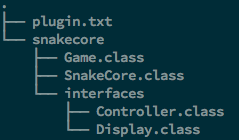
\includegraphics{ressources/plugin-organization.png}
   \caption{Contenu d'une archive d'un plugin}
\end{figure}

Dans l'exemple ci-dessus, on remarque que le fichier de configuration 
\emph{plugin.txt} se trouve à la racine de l'archive. La classe principale de ce 
plugin est \emph{SnakeCore} dont le package est \emph{snakecore} ce qui se traduit 
par le fait que la classe se trouve dans le sous-répertoire \emph{snakecore}.
\\\\
Il s'agit d'un plugin runnable qui défini des interfaces -- \emph{Controller} et 
\emph{Display} -- et qui doit donc obligatoirement les placer dans le sous-package 
\emph{interfaces} se trouvant au niveau de la classe principale du plugin.

\section{Créer des plugins}
Le but de cette partie est de créer un plugin principal qui peut dire bonjour dans 
plusieurs langues. Le plugin principal \emph{Hello} sera chargé de dire bonjour et 
il va s'appuyer sur les plugins secondaires \emph{Francais} et \emph{Anglais} pour 
le dire dans ces deux langues.

\subsection{Générer le plugin principal}
Pour commencer, il est nécessaire de vérifier où le framework va chercher les 
plugins en regardant le fichier \emph{settings.txt}.
\\\\
L'équipe à mis à disposition le script \emph{createPlugin} dans le répertoire 
\emph{/plugins} et nous allons l'utiliser pour générer un projet maven pour notre 
plugin.

\begin{lstlisting}[language=bash,caption=Création du plugin hello]
$ ./createPlugin.sh 
This script will create a plugin skeleton for MGS framework

Your plugin name (will be folder name):
hello

Is it a runnable plugin ? (y or n)
y

Full qualified name of your plugin class (like com.plugin.MyPlugin):
com.hello.Hello

Plugin description:
Plugin principal qui dit bonjour

Generating plugin skeleton....
Plugin hello has been created in current directory
\end{lstlisting}

\subsection{Créer le patron pour les plugins secondaires}
Comme expliqué précédemment (voir \ref{sss:DetailsRunnable}), il est possible de 
définir des plugins secondaires qui seront utilisés par le plugin principal. 
Tout d'abord, il faut commencer par définir le périmètre fonctionnel des 
plugins secondaires que l'on veut à travers une interface.
\\\\
Pour cela il faut créer le package \emph{interfaces} au niveau de la classe 
principale du plugin et à l'intérieur définir notre interface \emph{Speak} qui 
permet de dire bonjour.

\lstset{language=java,caption=/plugins/hello/src/main/java/com/hello/interfaces/Speak.java}
\lstinputlisting{ressources/Speak.java}

\subsection{Générer les plugins secondaires}
Nous allons de nouveau utiliser le script \emph{createPlugin} pour générer les 
projets pour les plugins.

\begin{lstlisting}[language=bash,caption=Création du plugin francais]
$ ./createPlugin.sh 
This script will create a plugin skeleton for MGS framework

Your plugin name (will be folder name):
francais

Is it a runnable plugin ? (y or n)
n

Full qualified name of plugin category (like com.plugin.interface.MyInterface):
com.hello.interfaces.Speak

Full qualified name of your plugin class (like com.plugin.MyPlugin):
com.francais.Francais

Plugin description:
Plugin secondaire pour hello, dit bonjour en francais

Generating plugin skeleton....
Plugin francais has been created in current directory
\end{lstlisting}

Il faut maintenant définir l'action du plugin lorqu'on lui demande de dire bonjour. 
Pour ce faire il faut compléter le code de la méthode \emph{sayHello} founie par 
l'interface \emph{Speak}.

\lstset{language=java,caption=/plugins/francais/src/main/java/com/francais/Francais.java}
\lstinputlisting{ressources/Francais.java}

La création du plugin \emph{Anglais}, se fait exactement de la même manière à ceci 
près qu'il faut attention au nom du plugin et à celui de la classe principale.

\subsection{Compilation et réglages du framwork}
Nous avons à cette étape nos trois plugins \emph{hello}, \emph{francais} et 
\emph{anglais} qui sont créés et implémentés mais il faut maintenant les compiler 
pour ensuite les importer dans la plateforme.

\begin{lstlisting}[language=bash,caption=Compilation des plugins]
$ cd /plugins/hello
$ mvn install

$ cd /plugins/
$ ./importPluginsOnPlatform.sh
\end{lstlisting}

Avant d'importer les plugins il est nécessaire d'installer le plugin principal 
afin de pouvoir satisfaire la dépendance des plugins secondaire par rapport 
à ce dernier.
\\\\
Un fois l'importation terminée, tout les plugins seront présents -- sous la forme 
d'archives \emph{jar} -- dans le répertoire \emph{/platform/resources/plugins/}.

La dernière chose à faire est de dire au framework de démarrer notre plugin 
\emph{hello} au démarrage. Pour cela, il faut renseigner le nom du plugin 
-- nom du fichier .jar -- dans le paramètre \emph{startplugin} du fichier de 
configuration du framework.

\section{Appels au framework}
Etant donné qu'un plugin principal peut utiliser des plugins secondaires gérés 
par le framework, il est possible d'instancier des plugins secondaires à 
partir d'un plugin principal.
\\\\
La classe \emph{Hello} du plugin \emph{hello} hériter de la classe 
\emph{MGSApplication} et c'est ce lien qui va permettre de faire des appels au 
framework. 
\\\\
En fait, nous avons fait ce choix car l'utilisation d'un singleton aurait pu 
donner accès au framework à n'importe quel plugin (même secondaire). De plus, si 
nous avions choisi de passer l'accès en paramètre de la fonction surchargée -- 
\emph{run} -- ceci aurait obligé l'utilisateur à ajouter un attribut pour stocker 
l'accès au framework.
\\\\
Cette classe possède deux attributs directement accessibles par le plugin :
\emph{currentPlugin} et \emph{pluginLoader}. Le premier regroupe tout simplement 
la configuration du plugin courant -- hello -- mais le second donne accès au 
gestionnaire de plugins.

\begin{table}[h]
	\begin{tabular}{|l|}

		\hline
		\texttt{Collection<RunnablePlugin> getRunnablePluginsList()}\\
		\hline
		Tout les plugins principaux (runnable)\\
		\hline

		\hline
		\texttt{Collection<Plugin> getClassicPlugins()}\\
		\hline
		Tout les plugins secondaires chargés par le framework (exepté les \\
		plugins	principaux).\\
		\hline
			
		\hline
		\texttt{List<Plugin> getClassicPluginsByCategory(String category)}\\
		\hline
		Tout les plugins secondaires ayant la catégorie donnée\\
		\hline			
			
		\hline
		\texttt{Object loadPlugin(Plugin plugin) throws IOException}\\
		\hline
		Charge le plugin donné en paramètre. Cette fonction assure que le plugin\\
		retourné est bien une sous-classe de sa catégorie.\\
		\hline
		
		\hline
		\texttt{Object loadPlugin(String pluginName) throws IOException}\\
		\hline
		Cette méthode réutilise la précédente mais permet de ne charger un plugin\\
		à partir du nom de son archive jar. Lance une exception si le plugin demandé\\
		n'existe pas\\
		\hline		
	\end{tabular}	
\caption{Méthodes du gestionnaire de plugins}
\end{table}

\section{Fonctionnement interne}
Lors d'une première phase, le framework va lire le fichier de configuration -- 
\emph{settings.txt} -- pour trouver le chemin vers le dossier des plugins. 
Ensuite, il va scanner les jars, lire le fichier de configuration 
\emph{plugins.txt} et stocker la liste des plugins dont la configuration est valide.

\begin{quote}
	\textbf{Attention !} Le framework indique au démarrage pour chaque plugin 
	s'il a été chargé ou non. 
	\\\\
	Certaines propriétés du fichier \emph{plugin.txt} sont déduites par le 
	framework: \emph{runnable} est faux par défaut et ce n'est pas obligé de 
	donner la \emph{category} pour un plugin principal car c'est toujours la 
	même (voir \ref{tab:plugintxt}).
\end{quote}

Une fois cette étape de chargement de la liste des plugins, le framework va 
démarrer le plugin par défaut qui a été indiqué avec \emph{startplugin} dans son 
fichier de configuration. Tout de fois, si le fichier de configuration du 
framework indique l'utilisation du mode debug ce sera l'inspecteur de plateforme 
qui sera lancé.

\section{Outils de la plateforme}
\subsection{Importation des plugins}
Tout les plugins que la platforme utilise doivent être placés dans son sous-
répertoire \emph{resources/plugins} sous forme d'archives jar.
\\\\
Pour faciliter le développement et l'installation de tout les plugins d'un seul 
coup nous avons créer le script bash \emph{/plugins/importPluginsOnPlatform.sh}.
Ce dernier permet de compiler tout les plugins et de les importer automatiquement
dans la platforme.
\\\\
Il est possible de passer un argument -- nom du dossier d'un plugin -- afin de 
préciser le plugin qui doit etre importé afin d'éviter de tout les importer
à chaque fois.

\subsection{Patrons de plugins}
Au cours du développement, nous avons fait le choix d'utiliser \emph{maven} 
pour gérer chaque projet représentant un plugin. Le script 
\emph{/plugins/createPlugin.sh} permet de générer de manière automatique un 
projet maven pour démarrer le développement d'un nouveau plugin.
\\\\
Les informations à propos du plugins sont demandés de manière interactive ce
qui permet d'annuler à tout moment la création du plugin.

\subsection{Inspecteur de plateforme}
Nous avons créer un plugin -- utilisant notre platforme -- qui sous la forme
d'une interface graphique permet de visualiser les réglages de la plateforme.
\\\\
En plus d'afficher le contenu du fichier \emph{/platform/resources/settings.txt}, 
cet outil donne la liste de tout les plugins principaux que la plateforme
est capable de charger. L'interface montre également la configuration de ces plugins
ainsi que les interfaces définies et les plugins secondaires les utilisant.
\\\\
Il est possible à tout moment, de lancer un plugin principal à partir de cet outil 
et celui-ci se lancera de manière automatique si le fichier de configuration 
de la plateforme indique que le mode \emph{debug} est actif.

\end{document}